\documentclass[a4paper]{jpconf}
\bibliographystyle{iopart-num}
\usepackage{amsmath}
\usepackage{citesort}
\usepackage{subfigure}
\usepackage{graphicx}
\graphicspath{{fig/}}
\usepackage{ifpdf}
\ifpdf\usepackage{epstopdf}\fi
\usepackage[export]{adjustbox}

%----------------------------------------------------- 
%\usepackage{soul,ulem,color,xspace,bm}
% Suggest to remove
%\newcommand{\asrm}[1]{{\color{magenta}\sout{#1}}}
% Suggest to insert
%\newcommand{\as}[1]{\color{cyan}#1\xspace\color{black}}
% Suggest to replace
%\newcommand{\asrp}[2]{\asrm{#1} \as{#2}}
% Comment
%\newcommand{\ascm}[1]{{\color{green}\;AS: #1}}
%------------------------------------------------------

\begin{document}
\title{Modelling of electron acceleration in relativistic supernovae}

\author{V I Romansky$^{1}$, A M Bykov$^{1,2}$ and S M Osipov$^1$}

\address{$^1$ Ioffe Institute, 26 Politekhnicheskaya st., St. Petersburg 194021, Russia}
\address{$^2$ Peter the Great St.~Petersburg Polytechnic University, 29 Politekhnicheskaya st., St. Petersburg 195251, Russia}

\ead{romanskyvadim@gmail.com}

\begin{abstract}
	Modern observations with high angle resolution of radio emission in supernova remnants show that there exists type of objects, expanding with velocities close to speed of light. Model of electron acceleration is necessary for reasonable interpretation of this observations. In this paper we present numerical Particle-in-Cell simulation of relativistic shock wave propagating in turbulent medium.
\end{abstract}
\section{Introduction}
Shock waves in supernova remnants are possible sources of cosmic rays. The process of acceleration on the shock front is nonlinear problem and it's efficiency depends on large number of factors. In this work we studied the trans-relativistic shocks because they are probably the most effective. Energy that particle gains when crosses the shock front increases with shock velocity, but in ultra-relativistic shocks only small fraction of particles can return from downstream and efficiency is relatively low. In trans-relativistis shocks, with Lorentz-factor about 1.5, energy is high and particles still can return from downstream and cross shock many times. Another problem is that due to Lorentz transformation perpendicular component of magnetic field growths and shock wave becomes quasi-perpendicular for majority of fields inclination angles. Quasi-perpendicular shock waves are very weak sources of accelerated particles as shown in . We introduce turbulent field in plasma medium to make shock wave quasi-parallel in some regions and make acceleration process more efficient.

\section{Numerical setup}
We studied evolution of quasi-perpendicular trans-relativistic shock, propagating in turbulent medium, and spectra of accelerated particles. The simulation is two dimensional, with three dimensional velocities and fields. Plasma flows into the simulation region through the right boundary, and reflects on the super-conducting wall at the left boundary. We used following parameters for setup: the initial flow Lorentz factor $\gamma = 1.5$, magnetization $\sigma = \frac{B^2}{4\pi\gamma (n_p m_p + n_e m_e) c^2} = 0.04$, in turbulent case $B^2$ means mean square field. The temperature $T = 5\cdot10^8 \rm{K}$ and proton mass is reduced to $m_p = 25 m_e$. Size of simulation region along x axis is $Lx = 8000\frac{c}{\omega_p}$ and in transverse direction $Ly = 200\frac{c}{\omega_p}$, where $\omega_p$ is plasma frequency $\omega_p = \sqrt{\frac{4\pi q^2 n}{\gamma m_e}}$. This sizes correspond to $80000$ and $2000$ grid points respectively. Also, $2000$ grid points corresponds to approximately $10$ gyroradii of upstream protons.
We initialize turbulent field via following formula: 
\begin{equation}
B_{turb} (x) = \sum_{i=0}^{n}\sum_{j=0}^{n}\sum_{p=1,2}B(k_x(i),k_y(j)) \textbf{e}_{p} sin(k_x(i) + k_y(j) + \phi (i,j,p))
\end{equation}
where $B(k_x(i),k_y(j))$ is amplitude of turbulent mode, usually we choose $B \propto k^{-5/3}$ and normalized to fixed fraction of total magnetic energy, $\eta$. $\textbf{e}_{p}$ are vectors corresponding to two different field polarizations and $\phi (i,j,p)$ is randomly generated phase for each mode. Wave vectors $k$ are distributed on uniform grid, $k_x = i \Delta k, k_y = j \Delta k$ and $\Delta k \approx \frac{2 \pi}{10 r_g}$ where $r_g$ is upstream proton gyroradius. And the maximum wavevector $k_{max} \approx \frac{2 \pi}{r_g}$. This equations are evaluated in plasma rest frame and then magnetic field is transformed to the downstream frame.

In this work we used setups with different turbulence scales, fraction of turbulent energy and regular field orientation and studied how this parameters influence on accelerated particles spectra.
\section{Results}


Simulation shows that structure of shock wave and velocity of it's propagation depends on properties of turbulence in upstream flow. On Figures \ref{regularB}, \ref{turbulentB} one can see relation of magnetic field in shock wave to upstream regular field. In case of strong turbulence in upstream, in downstream also exists strong turbulence. Shock front moves slowly and seems to be coorugated.

\begin{figure}[h!]
	\centering
	\begin{minipage}{0.49\textwidth}
		\centering
		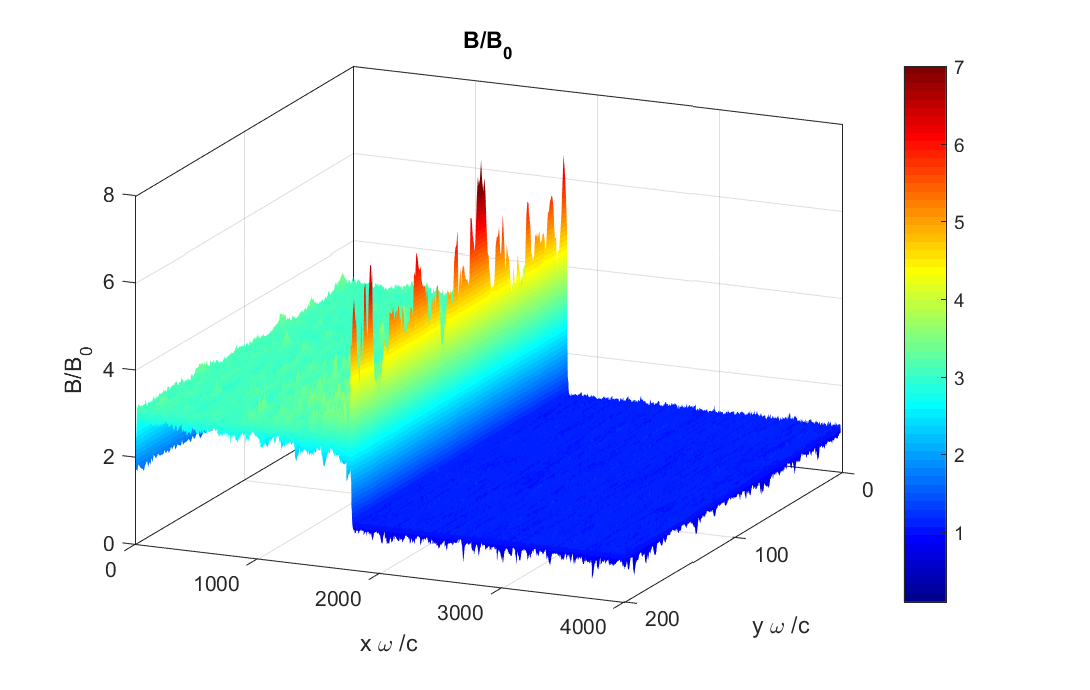
\includegraphics[width=0.98\textwidth]{fig/regular_field.eps} 
		\caption{Magnetic field in shock wave without turbulence.}
		\label{regularB}
	\end{minipage}\hfill
	\begin{minipage}{0.49\textwidth}
		\centering
		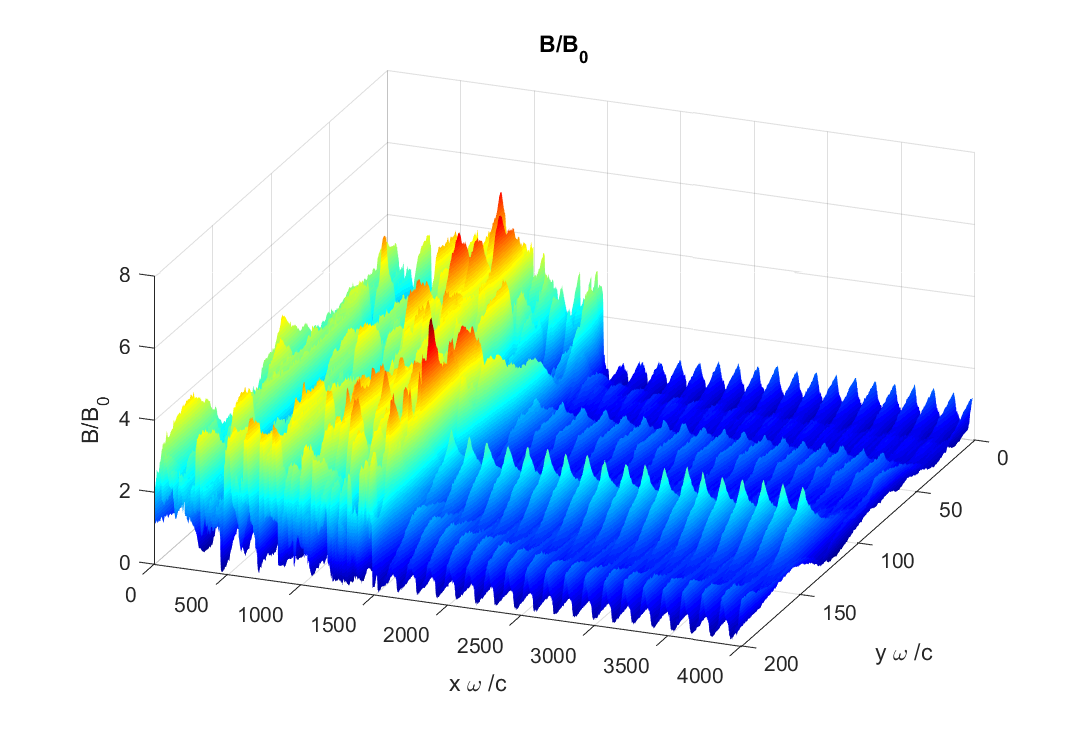
\includegraphics[width=0.98\textwidth]{fig/turbulent_field.eps} 
		\caption{Magnetic field in shock wave with 90\% turbulence.}
		\label{turbulentB}
	\end{minipage}
\end{figure}
Spectrum of accelerated electrons shows strong dependence on fraction of turbulent magnetic field, as shown on in Figure \ref{spectrum}. When half of energy is in turbulence, spectrum becomes significantly different from spectrum in regular field. Fraction of accelerated electrons highly increases with growth of turbulent energy fraction. 

\begin{figure}[h!]
	\centering
	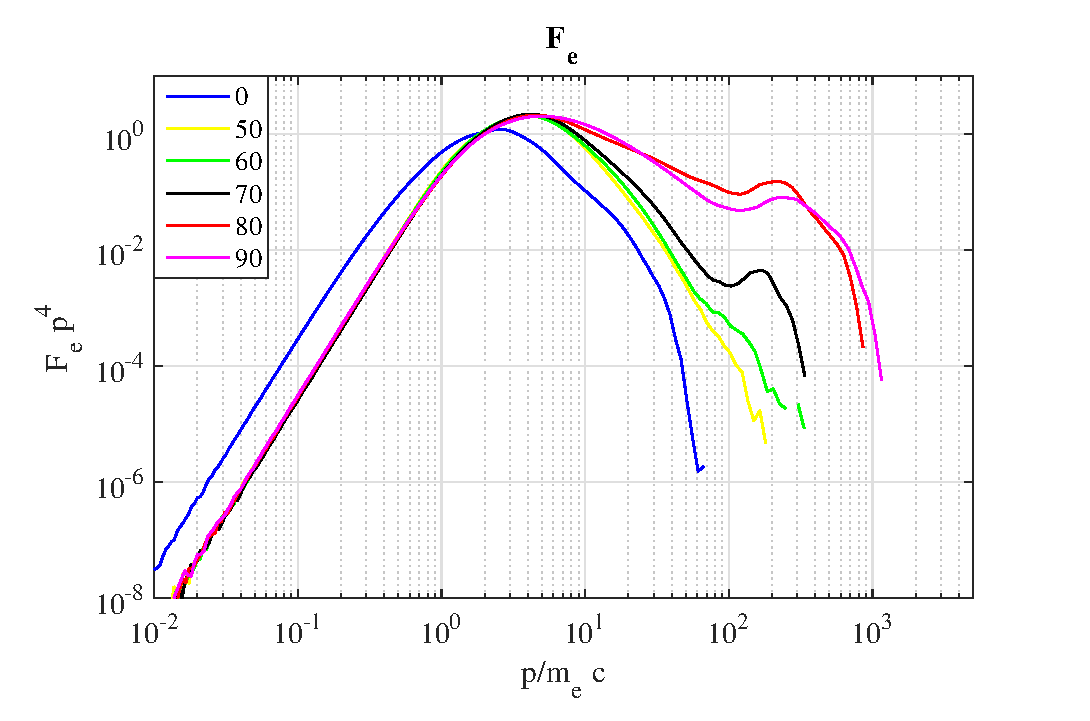
\includegraphics[width=0.8\textwidth]{fig/spectrum.eps} 
	\caption{Distribution of electrons in the relativistic shock wave with different turbulence fractions.}
	\label{spectrum}
\end{figure} 

\section{Conclusions}

\ack

The numerical results presented here were obtained using computational resources of Peter the Great Saint-Petersburg Polytechnic University Supercomputing Center (http://www.scc.spbstu.ru). 

\section*{References}
\begin{thebibliography}{20}
	\bibitem{Bell1978} Bell A R 1978 \textit{MNRAS} \textbf{182} 147
	\bibitem{Blandford1978} Blandford R D and Ostriker J P 1978 \textit{ApJ} \textbf{221} L29 
	\bibitem{Bykov2014} Bykov A M, Ellison D C, Osipov S M and Vladimirov A E 2014 \textit{ApJ} \textbf{789} Issue 2, 137
	\bibitem{Berezhko2003} Berezhko E G, Ksenofontov L T and V{\"o}lk H J  2003 \textit{A}{\&}\textit{A} \textbf{412} L11
	\bibitem{Uchiyama2007} Uchiyama Y, Aharonian F A, Tanaka T, Takahashi T and Maeda Y 2007 \textit{Nature} \textbf{449} 576
	\bibitem{Romansky2016} Romansky V I, Bykov A M, Osipov S M and Gladilin P E 2017 \textit{Journal of Physics: CS} \textbf{929} id 012014 
	\bibitem{Lapenta2006} Lapenta G, Brackbill J U and Ricci P 2006 \textit{Phys. Plasmas} \textbf{13} 055904
	\bibitem{Noguchi2007} Noguchi K, Tronci C, Zuccaro G and Lapenta G 2007 \textit{Phys. Plasmas} \textbf{14} 042308
	\bibitem{Ellison2013} Ellison D C, Warren D C and Bykov A M 2013 \textit{ApJ} \textbf{776} Issue 1, 46
	\bibitem{Pelletier2017} Pelletier G, Bykov A M, Ellison D C and Lemoine M 2017 \textit{Space Science Reviews} \textbf{207} Issue 1-4, pp. 319-360
	\bibitem{Sironi2011} Sironi L and Spitkovsky A 2011 \textit{ApJ} \textbf{741} Issue 1, 39
	\bibitem{Iwamoto2017} Iwamoto M, Amano T, Hoshino M and Matsumoto Y 2017 \textit{ApJ} \textbf{840} Issue 1 article id. 52, 14 pp.
	\bibitem{Margutti} Margutti R et al. 2014 \textit{ApJ}. \textbf{797} Issue 2, article id. 107 8 pp.
	\bibitem{Buneman} Buneman O 1993 \textit{Computer Space Plasma Physics} Terra Scientific Tokyo  67 p.
	\bibitem{Crumley} Crumley P, Caprioli D, Markoff S and Spitkovsky A \textit{MNRAS} \textbf{485} Issue 4, pp. 5105-5119
	
\end{thebibliography}
\end{document}